\documentclass[11pt]{article}
\usepackage{amsmath,amsfonts,mathabx}
\usepackage{graphicx}
\usepackage{hyperref}

% PREAMBLE
\newcommand{\RR}{\ensuremath{\mathbb{R}}}
\newcommand{\RRn}[1]{\mathbb{R}^{#1}}
\DeclareMathOperator{\function}{function}

% Code listing
\usepackage[listings]{tcolorbox}


\begin{document}


\begin{center}
{\textbf{\LARGE Chapitre 4: Mod\`eles de r\'egression pour donn\'ees binaires}}
\end{center}

\noindent Les mod\`eles vus dans les deux chapitres pr\'ec\'dents ne permettent de consid\'erer que les cas o\`u la variable r\'eponse $Y_i$ est continue, pusiqu'on supposait  que $Y_i$ suivait une loi normale. Cependant, dans plusieurs situation, on a une variable r\'eponse discr\`ete qui ne peut prendre qu'un nombre fini (ou d\'enombrable) de valeurs possibles. Dans ce chapitre, on s'int\'eresse au cas o\`u $Y_i$ suit une loi de Bernoulli ou une loi binomiale. Voici quatre exemples:
\begin{enumerate}
\item[{\bf Ex 1:}] Consid\'erons le jeu de donn\'ees \textsf{quilpie} de la library \texttt{GLMsData} du logiciel \textrm{R}. Ce jeu de donn\'ees contient des observations de 1921 \`a 1988 de la quantit\'e de pluie mesur\'ee durant le mois de juillet \`a Quilpie en Australie. Le jeu de donn\'ees contient des variables explicatives qui concernent la pression atmosph\'erique. La variable r\'eponse ne peut prendre que 2 valeurs: 1 si la quanti\'e de pluie mesur\'ee est sup\'erieure \`a 10 millim\`etres et 0 sinon.
\item[{\bf Ex 2:}] Consid\'erons le jeu de donn\'ees \textsf{nminer} de la library \texttt{GLMsData} du logiciel \textrm{R}. Ce jeu de donn\'ees contient 31 observations de 9 variables. La variable r\'eponse \textsf{Mminers} ne peut prendre que 2 valeurs: 1 si un mineur bruyant est d\'etect\'e dans la parcelle de terre et 0 sinon.
\item[{\bf Ex 3:}] Consid\'erons le jeu de donn\'ees \textsf{deposit} de la library \texttt{GLMsData} du logiciel \textrm{R}. Ce jeu de donn\'ees contient 18 observations avec deux variables explicatives : type ($A$, $B$ ou $C$) et dose d'insecticide. La variable r\'eponse $Y_i$ est le nombre d'insectes tu\'es parmi les $m_i$ insectes vivants au d\'ebut de l'exp\'erience.
\item[{\bf Ex 4:}] Consid\'erons le jeu de donn\'ees \textsf{turbines} de la library \texttt{GLMsData} du logiciel \textrm{R}. Ce jeu de donn\'ees contient 11 observations avec une variable explicative : nombre d'heures de fonctionnement. La variable r\'eponse $Y_i$ est le nombre machines qui pr\'esentent des fissures parmi les $m_i$ machines neuves au d\'ebut de l'exp\'erience.
\end{enumerate}

\section{Donn\'ees et mod\`ele}

\subsection{Donn\'ees individuelles}

\noindent Dans les deux premiers exemples, la variable r\'eponse $Y_i$ ne peut prendre 	que deux valeurs possibles: 0 et 1. Les donn\'ees sont donc sous la forme $\{(Y_i,X_i), i=1,\cdots,n\}$; o\`u $n$ est nombre d'oservations, $Y_i \in \{0,1\}$ est la variable r\'eponse et $X_i=(X_{i1},\cdots,X_{ip})^\top$ est l'ensemble des variables explicatives pour l'observation $i$. On dit que $Y_i$ suit une loi de Bernoulli avec un param\`etre $pi_i \in [0,1]$. On pose alors $P(Y_i=1)=\pi_i$ et $P(Y_i=0)=1-P(Y_i=1)=1-\pi_i$ et on a

\begin{eqnarray*}
P(Y_i=y_i)&=& \pi_i^{y_i}(1-\pi_i)^{1-y_i}, \, \, \, y_i \in \{0,1\}\\
E[Y_i] &=& \mu_i = \pi_i \\
Var[Y_i] &=& \sigma^2_i = \pi_i(1-\pi_i).
\end{eqnarray*}

\noindent D'autres part, on pose $\eta_i=\beta_0+\beta_1 X_{i1} + \cdots + \beta_p X_{ip}, i=1,\cdots,n$. Ici $p$ est le nombre de variables explicatives consid\'er\'ees et $\beta=(\beta_0,\beta_1,\cdots,\beta_p)^\top$ est un vecteur de $p+1$ coefficient de r\'egression. \`a estimer \`a parti des donn\'ees. 

\noindent Finalement, on a $\eta_i = g(\pi_i)$; o\`u $g(\cdot)$ est une fonction de lien, suppos\'ee connue. La fonction de lien la plus populaire est $$g(u)=\mbox{logit}(u)=\log\left(\frac{u}{1-u}\right).$$ 

\noindent Avec cette fonction de lien, on a 
$$\pi_i = P(Y_i = 1) = \frac{e^{\beta_0+\beta_1 X_{i1} + \cdots + \beta_p X_{ip}}}{1+e^{\beta_0+\beta_1 X_{i1} + \cdots + \beta_p X_{ip}}}.$$

\noindent Et donc, si $\beta_j>0$, une hause de $X_{ij}$ avec toutes les autres variables explicatives maintenues constantes augmentera la probabilit\'e $P(Y_i = 1)$. Si $\beta_j<0$, une hause de $X_{ij}$ avec toutes les autres variables explicatives maintenues constantes diminuera la probabilit\'e $P(Y_i = 1)$. Finalement, si $\beta_j=0$, alors $X_{ij}$ n'a pas d'effets sur la probabilit\'e $P(Y_i = 1)$.

\subsection{Donn\'ees group\'ees}

\noindent Dans les deux derniers exemples, la variable r\'eponse $Y_i$ peut prendre n'importe quelle valeur dans l'ensemble $\{0,1,\cdots,m_i\}$, o\`u $m_i$ est un entier connu \`a l'avance et qui varie d'une observation \`a une autre. 'A toute fin pratique, $m_i$ peut \^etre consid\'er\'e comme un nombre total d'expr\'eriences ind\'ependantes ayant deux r\'esultats possibles (succ\`es ou \'echec) et $Y_i$ est interpr\'et\'e comme le nombre de succ\`es parmi les $m_i$ exp\'eriences. Les donn\'ees sont donc sous la forme $\{(Y_i,m_i,X_i), i=1,\cdots,n\}$. On dit que $Y_i$ suit une loi Binomiale de param\`etres $m_i$ et $\pi_i \in [0,1]$ et on \'ecrit $Y_i \sim \mbox{Bin}(m_i,\pi_i)$. Selon cette loi, on a:
\begin{eqnarray*}
P(Y_i=y_i)&=& \binom{m_i}{y_i} \pi_i^{y_i}(1-\pi_i)^{m_i-y_i}, \, \, \, y_i \in \{0,1,\cdots,m_i\}\\
E[Y_i] &=& \mu_i = m_i \pi_i \\
Var[Y_i] &=& \sigma^2_i = m_i \pi_i(1-\pi_i) = \frac{\mu_i(m_i-\mu_i)}{m_i}.
\end{eqnarray*}

\noindent Pour relier la variable r\'eponse aux variables explicative, on pose $\eta_i=g(\pi_i), i=1,\cdots,n$. Ce choix est motiv\'e par le fait que $\pi_i$ doit appartenir \`a l'intervalle $[0,1]$.

\noindent Si on a $m_1=m_2=\cdots=m_n=1$, on retrouve la loi de Bernoulli des deux premiers exemples. La loi de Bernoulli est un cas particulier de la loi binomiale. Dans la suite de ce chapitre, on se contentera de pr\'esenter les d\'eveloppements pour la loi binomiale.

\subsection{Fonctions de lien}

La fonction de lien $g$ sp\'ecifi\'ee pour des donn\'ees binaires doit s'assurer que $\pi_i=g^{-1}(\eta_i)$ appartient \`a l'intervalle $[0,1]$, puisque $\pi_i$ est une probabilit\'e. Trois fonctions de lien sont commun\'ement utilis\'ees pour les donn\'ees binaires:
\begin{enumerate}
\item[{\bf Logit:}] Cette fonction est d\'efinie par $$g(u)=\mbox{logit}(u)=\log\left(\frac{u}{1-u}\right).$$
\noindent Ainsi, on a $\pi_i=g^{-1}(\eta_i)=e^{\eta_i}/(1+e^{\eta_i})$. Avec logiciel \textrm{R}, on sp\'eficie \textsf{link="logit"} \`a l'int\'erieur de la fonction \textsf{glm}.
\item[{\bf Probit:}] Cette fonction est d\'efinie par $g(u)=\Phi^{-1}(u)$, o\`u $\Phi$ est la fonction de r\'epartition de la loi normale standard ${\cal N}(0,1)$.  Ainsi, on a $\pi_i=g^{-1}(\eta_i)=\Phi(\eta_i)$. Avec logiciel \textrm{R}, on sp\'eficie \textsf{link="probit"} \`a l'int\'erieur de la fonction \textsf{glm}.
\item[{\bf c-log-log:}] Cette fonction est d\'efinie par $g(u)=\log\{-\log(1-u)\}$. Ainsi, on a $\pi_i=g^{-1}(\eta_i)=1-e^{-e^{\eta_i}}$. Avec logiciel \textrm{R}, on sp\'eficie \textsf{link="cloglog"} \`a l'int\'erieur de la fonction \textsf{glm}.
\end{enumerate}

\noindent On remarque que dans les trois cas pr\'esent\'es ci-haut, $g^{-1}(\cdot)$ est une fonction de r\'epartition. 


\section{Inf\'erence statistique}

\subsection{Estimation des param\`etres $\beta$}
Le vecteur des param\`etres du mod\`ele est $\beta=(\beta_0,\beta_1,\cdots,\beta_p)^\top$. La fonction de log-vraisemblance est
\begin{eqnarray*}
\sum_{i=1}^n \log\left[P(Y_i=y_i)\right]&=&\sum_{i=1}^n \log\left[\binom{m_i}{y_i} \pi_i^{y_i}(1-\pi_i)^{m_i-y_i}\right] \\ 
&=& \sum_{i=1}^n \left\{\log\left[\binom{m_i}{y_i}\right]+y_i\log(\pi_i)+(m_i-y_i)\log(1-\pi_i)\right\}.
\end{eqnarray*}

\noindent Cette fonction d\'epent du vecteur de param\`etres $\beta$ \`a travers $\pi_i$, puisqu'on a 
$$\pi_i = g^{-1}(\eta_i) = g^{-1}(\beta_0+\beta_1 X_{i1} + \cdots + \beta_p X_{ip}).$$

\noindent En rempla\c{c}ant $\pi_i$ par $\mu_i/m_i$ dans l'expression pr\'ec\'edente, on montre que cette fonction log-vraisemblance est \'egale \`a
$$l(\mu;y) = \sum_{i=1}^n \left\{y_i \log(\mu_i) + (m_i-y_i) \log(m_i-\mu_i)\right\} + K$$

\noindent o\`u $$K = \sum_{i=1}^n \left\{\log\left[\binom{m_i}{y_i}\right] - m_i\log(m_i)\right\}$$
est une constante qui ne d\'epend pas de $\beta$. L'estimateur de maximum de vraisemblance de $\beta$, disons $\hat\beta$, est la valeur de $\beta$ qui maximise $l(\beta;y,\mu)$. On calcule par la suite la matrice d'information de Fisher $I$. L'\'el\'ement \`a la position $(j,k)$ de la matrice $I$ est \'egal \`a 
$$-\frac{\partial^2 l(\beta;y,\mu)}{\partial \beta_j \partial \beta_k}$$
\'evalu\'ee \`a $\beta=\hat\beta$. La matrice de variance-covariance de $\hat\beta$ est alors estim\'ee par $v(\hat\beta)=I^{-1}$. Par la th\'eorie g\'en\'erale de l'estimation par maximum de vraisemblance, la distribution asympotique de $\hat\beta$ est approxim\'ee par la loi normale multivari\'ee ${\cal N}\{\beta,v(\hat\beta)\}$.

\noindent On montre que $v(\hat\beta) = (X^\top W X)^{-1}$ o\`u $X$ est une matrice $n \times (p+1)$ contenant les variables explicatives, incluant l'intercepte et $W$ est une matrice diagonale de taille $n$ avec les entr\'ees $w_{i}=\hat\mu_i(m_i-\hat\mu_i)/m_i, i=1,\cdots,n$ sur la diagonale. Ici, on a
$$\hat\mu_i  = m_i \hat \pi_i = m_i g^{-1}(\hat\eta_i) = m_i g^{-1}(\hat\beta_0+\hat\beta_1 X_{i1} + \cdots + \hat\beta_p X_{ip})$$

\subsection{Tests d'hypoth\`eses et intervalles de confiance}
Les intervalles de confiances et les tests d'hypoth\`eses concernant les $\beta_j$ sont obtenus par la m\'ethode de Wald.

\noindent Ainsi, un intervalle de confiance \`a $100\times(1-\alpha)\%$ pour $\beta_j$ est donn\'e par $$[\hat\beta_j - z_{\alpha/2} \sqrt{v(\hat\beta_j)};\hat\beta_j + z_{\alpha/2} \sqrt{v(\hat\beta_j)}],$$
o\`u $z_{\gamma}$ est le quantile de la loi normale standard d\'efini par $P(Z>z_{\gamma})=\gamma$, $\gamma \in (0,1)$, $Z \sim {\cal N}(0,1)$ et $v(\hat\beta_j)$ est l'\'el\'ement $(j+1,j+1)$ de la matrice $v(\hat\beta)$, $j=0,1,\cdots,p$.

\noindent Consid\'erant maintenant le test d'hypoth\`ese $H_0: \beta_j = 0$ versus $H_1: \beta_j \neq 0$. On rejetter $H_0$ au seuil $\alpha$ si $|z_{obs}|>z_{\alpha/2}$, avec $z_{obs}=\hat\beta_j/\sqrt{v(\hat\beta_j)}$. Le seuil observ\'e ($p$-valeur ou $p$-value) est $\alpha^*=P(|Z|>|z_{obs}|)=2P(Z>|z_{obs}|)$, $Z \sim {\cal N}(0,1)$.

\noindent Int\'eressons nous maintenant \`a $\pi^*$ lorsque $X=X^*=(1,X_1^*,\cdots,X_p^*)^\top$. On estime $\pi$ par $\hat\pi^*=g^{-1}(\hat\beta_0+\hat\beta_1 X_{1}^* + \cdots + \hat\beta_p X_{p}^*)=g^{-1}(X^*\hat\beta)$.

\noindent Un intervalle de confinace \`a $100\times(1-\alpha)\%$ pour $X^*\beta$ est donn\'e par 
$$\left[ X^*\hat\beta - z_{\alpha/2}\sqrt{v(X^*\hat\beta)}   , X^*\hat\beta + z_{\alpha/2}\sqrt{v(X^*\hat\beta)}\right],$$

\noindent avec $v(X^*\hat\beta)=X^* v(\hat\beta) {X^*}^\top$. On en d\'eduit un intervalle de confiance \`a $100\times(1-\alpha)\%$ pour $\pi^*$:
$$\left[ g^{-1}\left\{X^*\hat\beta - z_{\alpha/2}\sqrt{v(X^*\hat\beta)}\right\},g^{-1}\left\{X^*\hat\beta + z_{\alpha/2}\sqrt{v(X^*\hat\beta)}\right\}   \right].$$

\noindent Alternativement, on peut approximer $Var(\hat\pi^*)$ par la r\`egle du delta. On obtient $v(\hat\pi^*)=h(X^*\hat\beta)v(X^*\hat\beta)$, o\`u $h(u)=\{\partial g^{-1}(u)/\partial u\}^2$. 

\noindent Un intervalle de confiance approximatif \`a $100\times(1-\alpha)\%$ pour $\pi^*$ est donn\'e par 
$$\left[\hat\pi^* - 1.96 \sqrt{v(\hat\pi^*)},\hat\pi^* - 1.96 \sqrt{v(\hat\pi^*)}\right].$$

\subsection{Exemple en R}

Consid\'erons le jeu de donn\'ees \textsf{turbines} de la library \texttt{GLMsData} du logiciel \textrm{R}.

\begin{verbatim}
> if (!require("GLMsData")) install.packages("GLMsData")
> library("GLMsData")#### Installer la librairie GLMsData
> 
> data(turbines)#### Rendre le jeu de donnees turbines disponible
> attach(turbines)
The following objects are masked from turbines (pos = 4):

    Fissures, Hours, Turbines

> 
> ##################################################################
> ## Ajustement du modele avec trois fonctions de lien differents ##
> ##################################################################
> 
> modele.logit <- glm(cbind(Fissures,Turbines-Fissures)~Hours,
                      data=turbines,family=binomial(link="logit"))
> modele.probit <- glm(cbind(Fissures,Turbines-Fissures)~Hours,
                       data=turbines,family=binomial(link="probit"))
> modele.cloglog <- glm(cbind(Fissures,Turbines-Fissures)~Hours,
                        data=turbines,family=binomial(link="cloglog"))
> 
> resultats <- round(rbind(summary(modele.logit)$coef,
                           summary(modele.probit)$coef,
                           summary(modele.cloglog)$coef),6)
> 
> resultats <- resultats[c(1,3,5,2,4,6),]
> 
> row.names(resultats) <- c("beta0 (logit)", "beta0 (probit)","beta0 (cloglog)",
                            "beta1 (logit)", "beta1 (probit)","beta1 (cloglog)")
> 
> resultats
                 Estimate Std. Error    z value Pr(>|z|)
beta0 (logit)   -3.923597   0.377959 -10.381013        0
beta0 (probit)  -2.275807   0.197419 -11.527823        0
beta0 (cloglog) -3.603280   0.324739 -11.095923        0
beta1 (logit)    0.000999   0.000114   8.753682        0
beta1 (probit)   0.000578   0.000063   9.238777        0
beta1 (cloglog)  0.000810   0.000090   8.992278        0
\end{verbatim}

\noindent Les trois fonctions de lien donnent des r\'esultats tr\`es similaires, ce qui est tr\`es fr\'equent.

\noindent Tra\c{c}ons maintenant $\hat\pi^*$ avec les intervalles de confiance pour diff\'erentes valeurs du nombre d'heures de fonctionnement. On utilise le lien logit et on calcule les intervalles de confiance de deux mani\`eres diff\'erentes, comme d\'etaill\'e ci-haut. Voici le code \textrm{R} pour la premi\`ere m\'ethode:

\begin{verbatim}
############################################################################
## On trace la courbe de pi predit en fonction du nombre d'heures         ##
## de fonctionnement avec les intervalles de confiance pour le lien logit ##
############################################################################

## 1ere facon: intervalles de confiance exacts

Heures <- 0:5000
nouvelles.donnees <- predict(modele.logit,
                     newdata=data.frame(Hours=Heures),se.fit=TRUE)
nu.chapeau <- nouvelles.donnees$fit
se.nu.chapeau <- nouvelles.donnees$se.fit
pi.chapeau <- exp(nu.chapeau)/(1+exp(nu.chapeau))
A <- exp(nu.chapeau-1.96*se.nu.chapeau)
B <- exp(nu.chapeau+1.96*se.nu.chapeau)
intervalle.confiance.1.pi.chapeau <- A/(A+1)
intervalle.confiance.2.pi.chapeau <- B/(B+1)

plot(Hours,Fissures/Turbines,xlab="Nombre d'heures de fonctionnement",pch=19,las=1,
     xlim=c(0,5000),ylim=c(0,0.7),ylab="Proportion de machines avec des fissures")
lines(Heures,pi.chapeau)
lines(Heures,intervalle.confiance.1.pi.chapeau,lty=2)
lines(Heures,intervalle.confiance.2.pi.chapeau,lty=2)
\end{verbatim}

\noindent et on obtient

\begin{center}
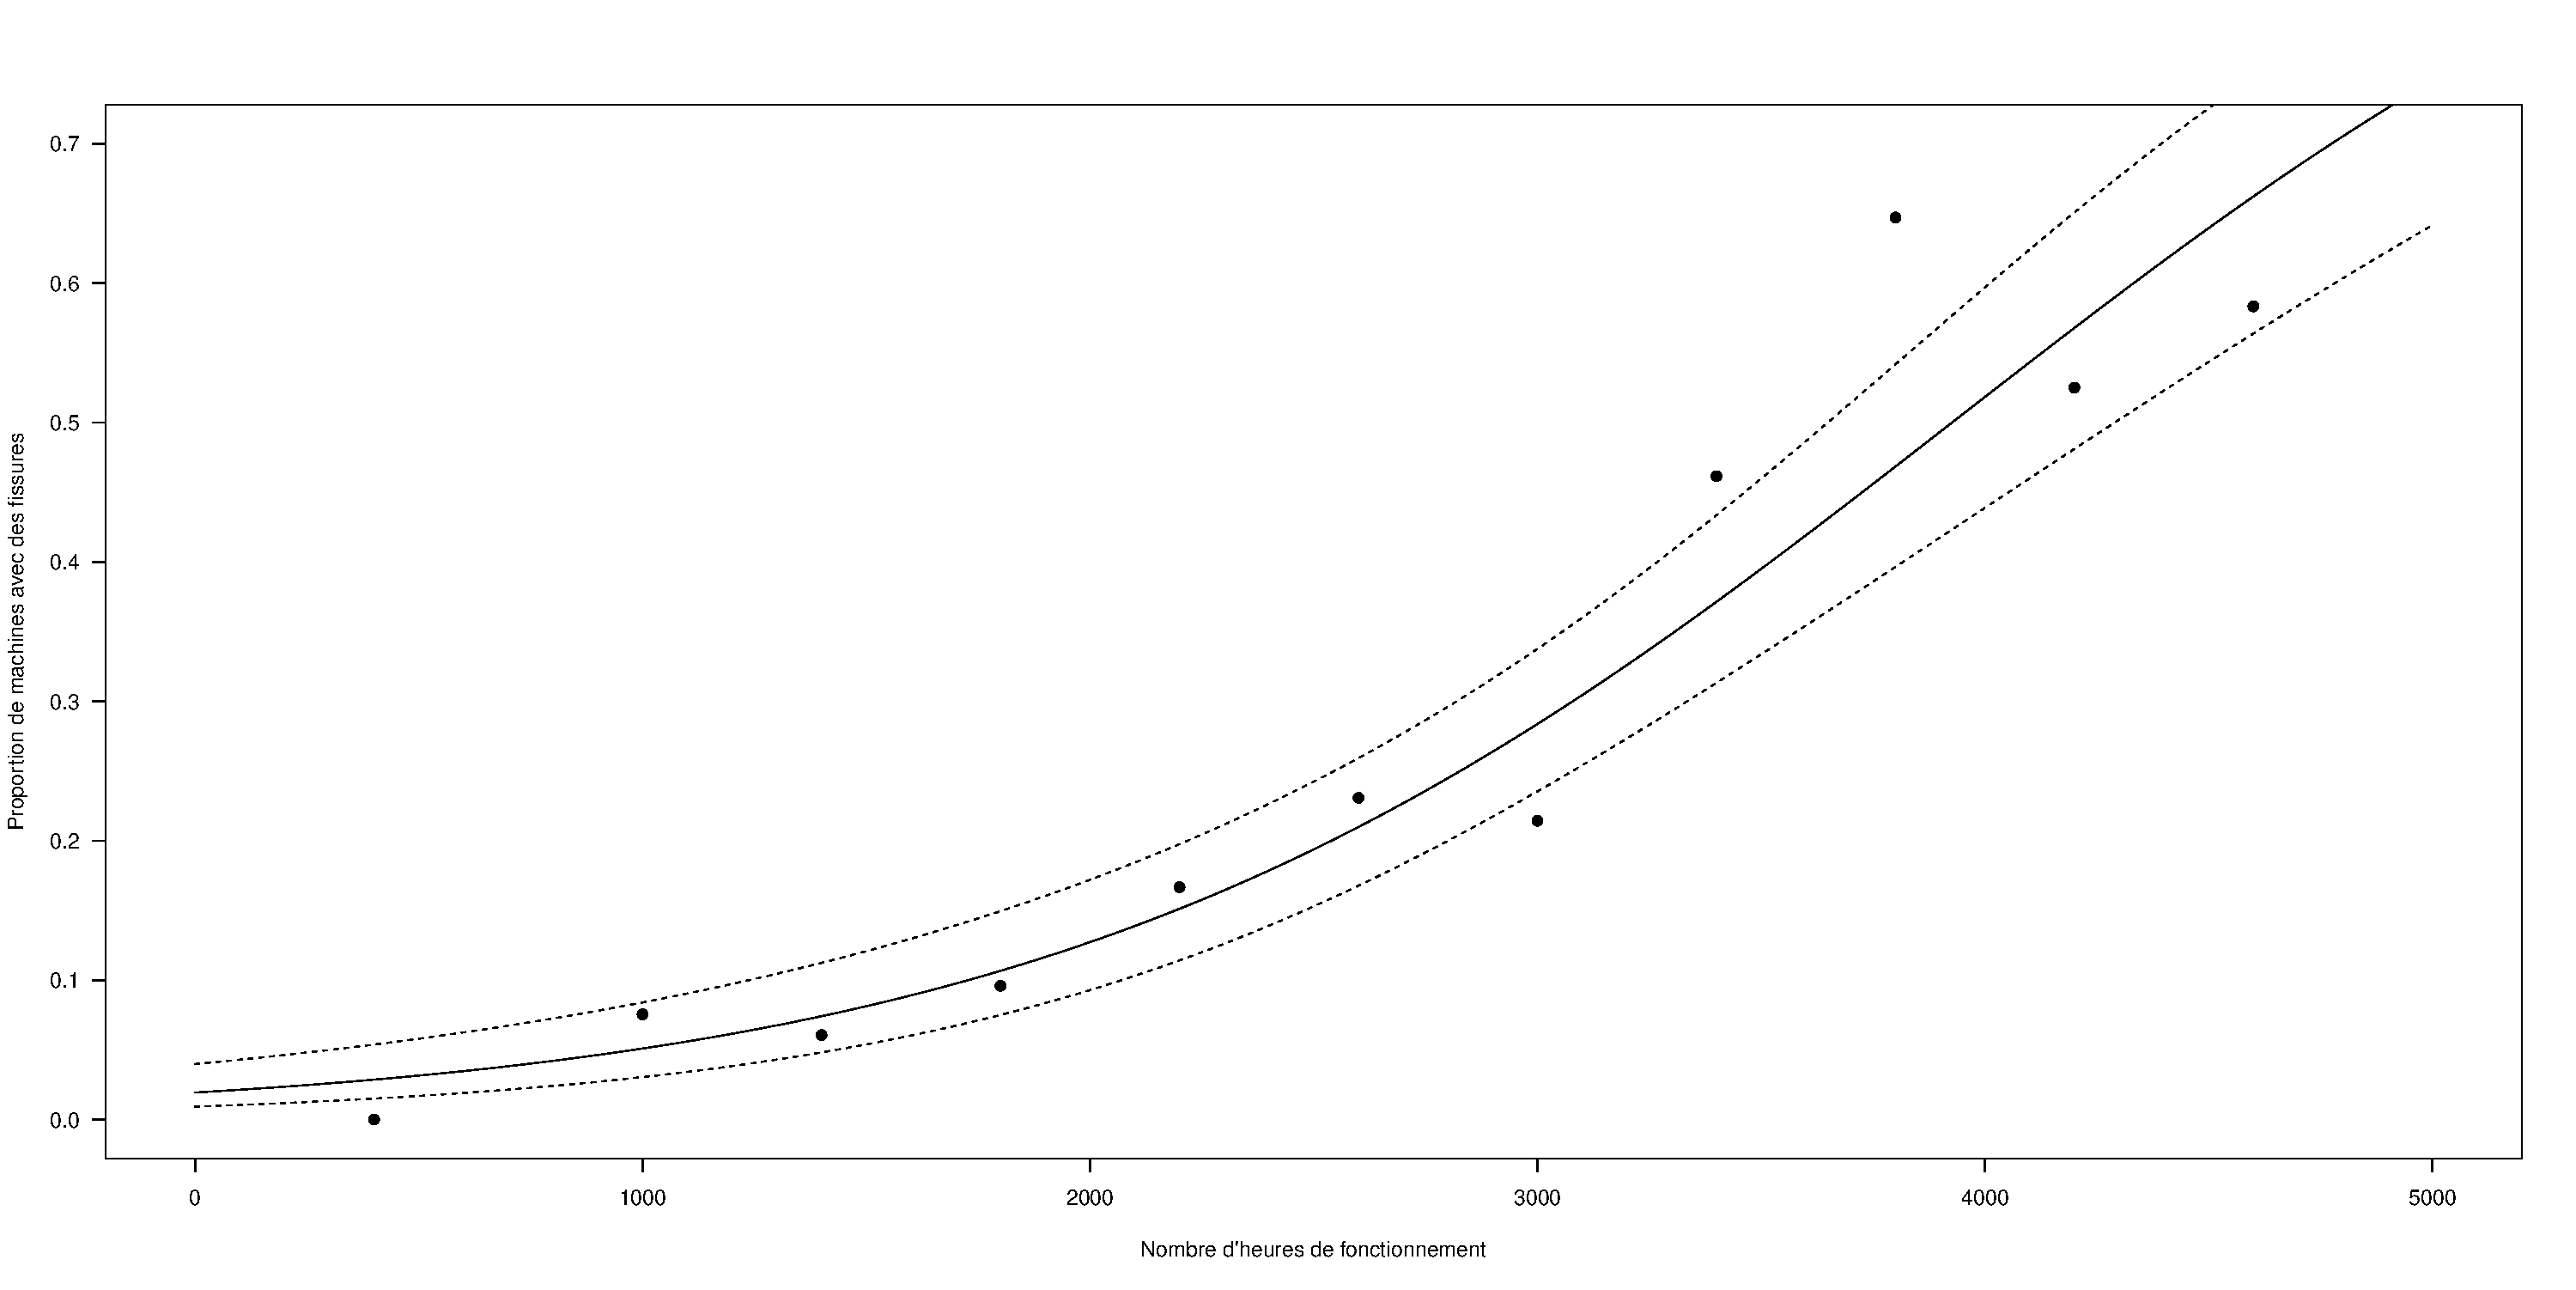
\includegraphics[scale=0.3]{Graphique2.pdf}
\end{center}

\noindent Et voici le code \textrm{R} pour la deuxi\`ere m\'ethode:

\begin{verbatim}
## 2eme facon: intervalles de confiance approximatifs

Heures <- 0:5000
nouvelles.donnees <- predict(modele.logit,newdata=data.frame(Hours=Heures),
                             se.fit=TRUE,type="response")
pi.chapeau <- nouvelles.donnees$fit
se.pi.chapeau <- nouvelles.donnees$se.fit
plot(Hours,Fissures/Turbines,xlab="Nombre d'heures de fonctionnement",pch=19,las=1,
     xlim=c(0,5000),ylim=c(0,0.7),ylab="Proportion de machines avec des fissures")
lines(Heures,pi.chapeau)
lines(Heures,pi.chapeau-1.96*se.pi.chapeau,lty=2)
lines(Heures,pi.chapeau+1.96*se.pi.chapeau,lty=2)
\end{verbatim}

\noindent et on obtient

\begin{center}
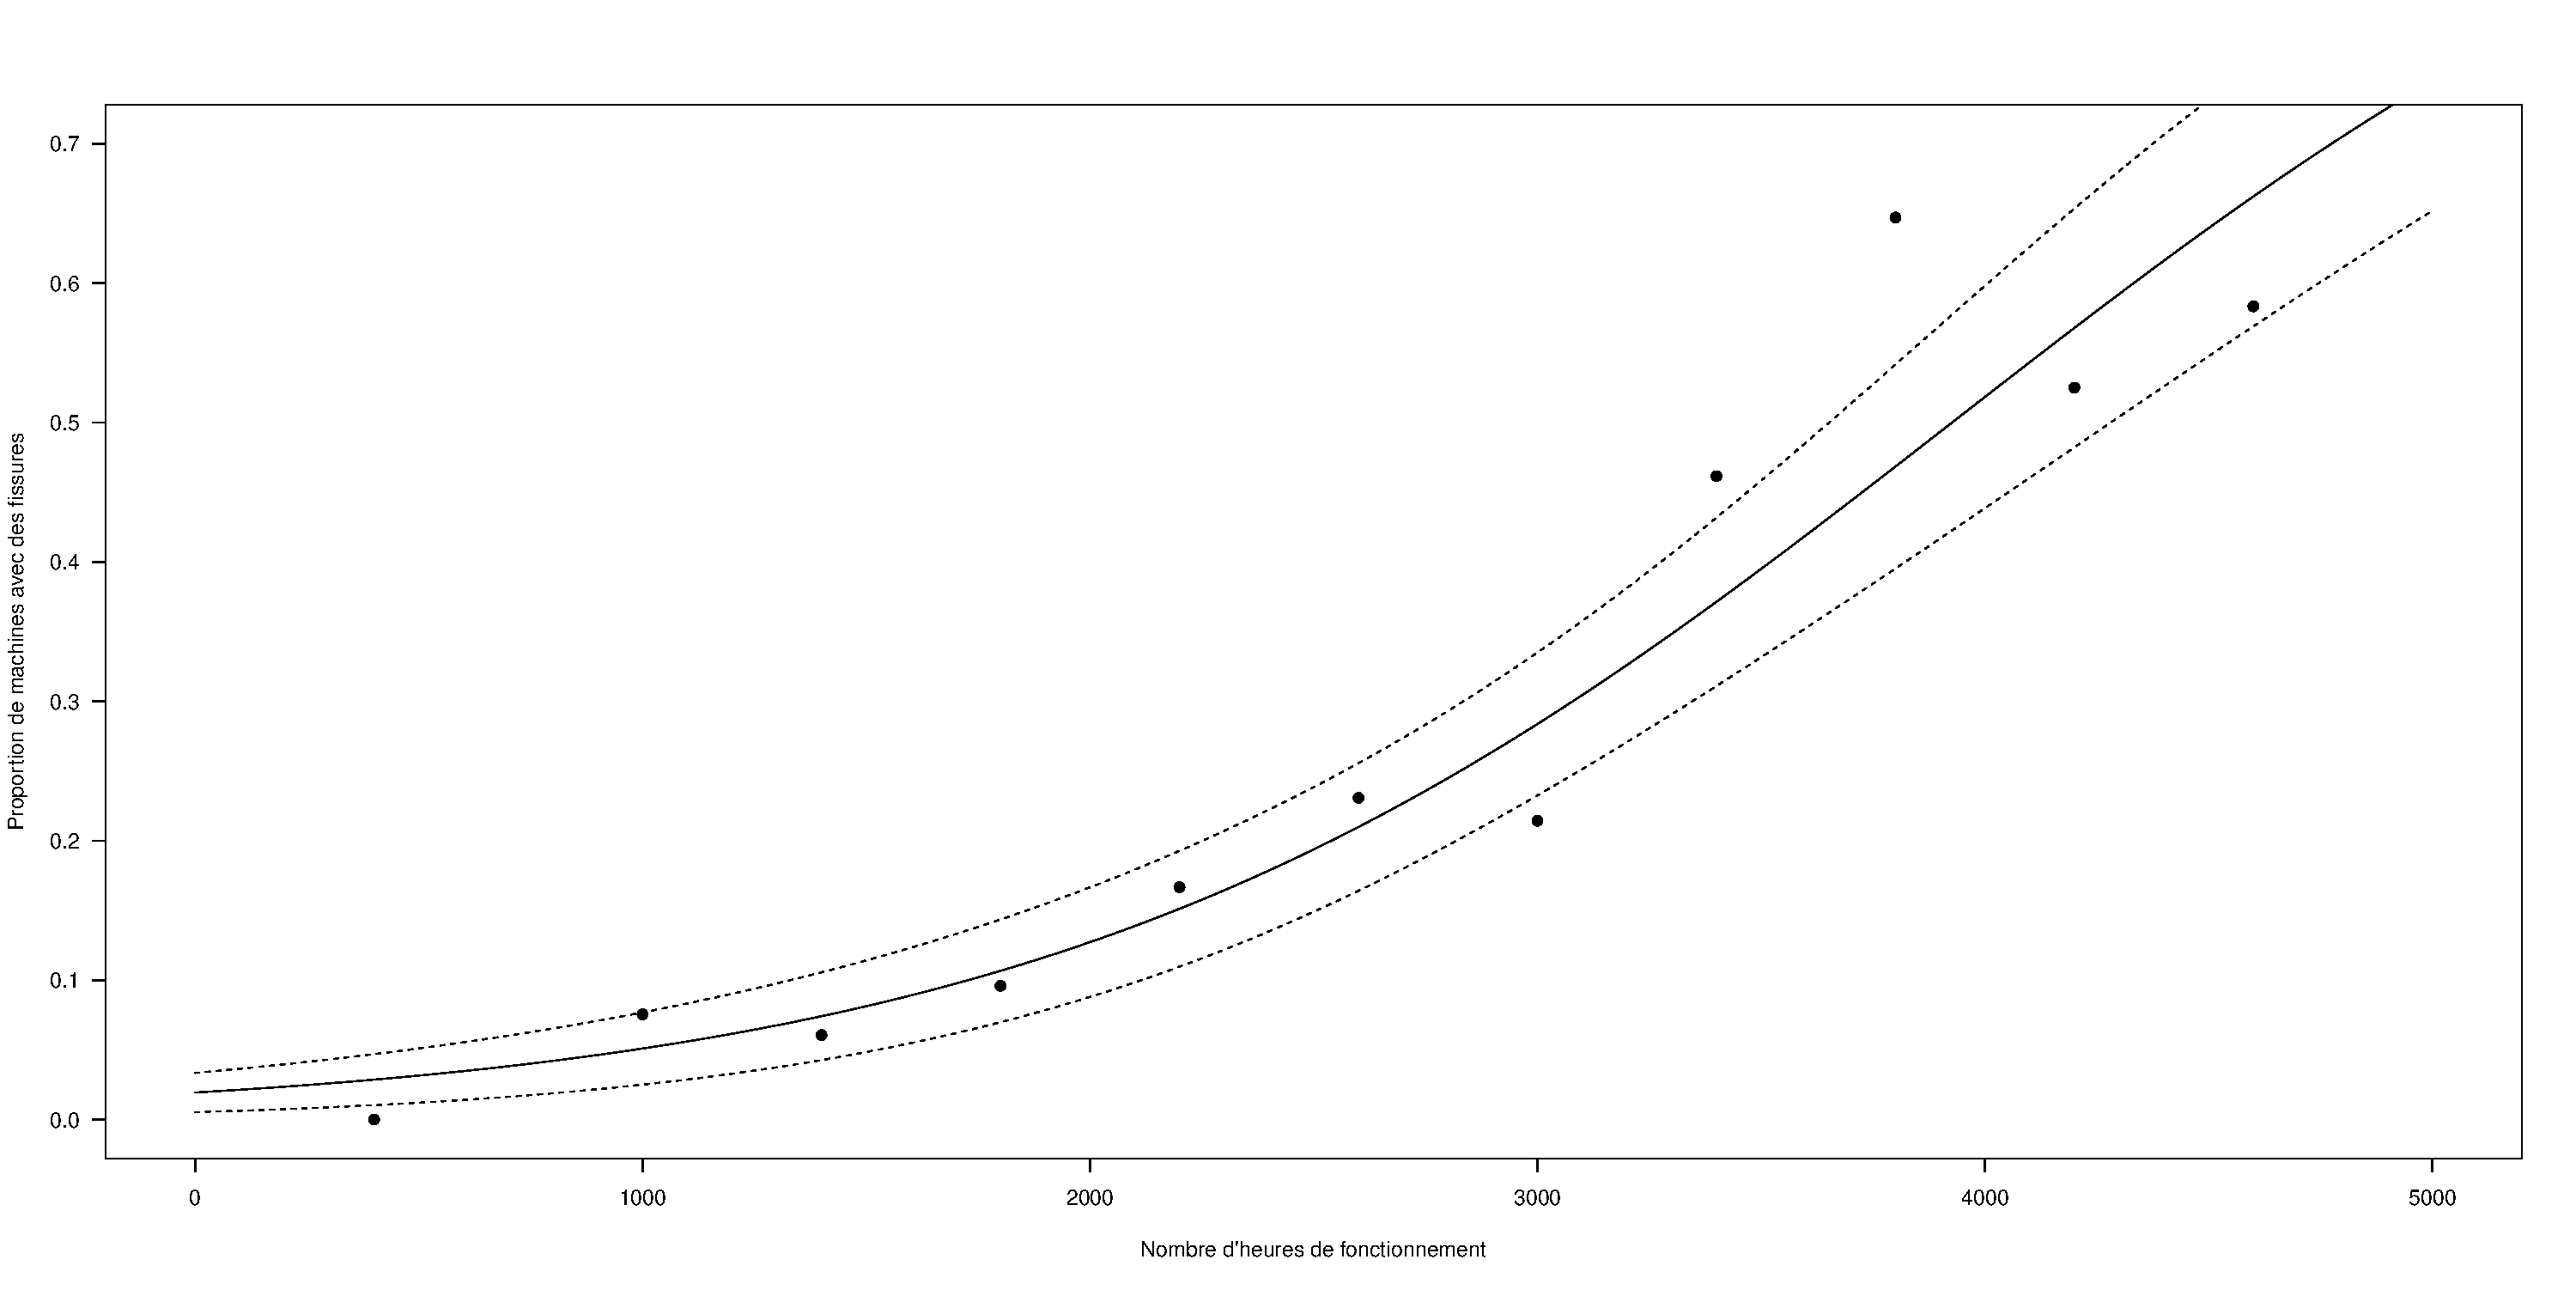
\includegraphics[scale=0.3]{Graphique3.pdf}
\end{center}

\noindent Les deux graphiques sont tr\`es similaires.

\noindent Tra\c{c}ons maintenant $\hat\pi^*$ pour diff\'erentes valeurs du nombre d'heures de fonctionnement en consid\'erant les 3 fonctions de lien.

\begin{verbatim}
###################################################################
## On trace la courbe de pi predit en fonction du nombre d'heure ##
## de fonctionnement pour les liens logit, probit et cloglog     ##
###################################################################

Heures <- 0:5000
nouvelles.donnees.logit <- predict(modele.logit,newdata=data.frame(Hours=Heures),
                                   se.fit=TRUE,type="response")
nouvelles.donnees.probit <- predict(modele.probit,newdata=data.frame(Hours=Heures),
                                    se.fit=TRUE,type="response")
nouvelles.donnees.cloglog <- predict(modele.cloglog,newdata=data.frame(Hours=Heures),
                                     se.fit=TRUE,type="response")
plot(Hours,Fissures/Turbines,xlab="Nombre d'heures de fonctionnement",pch=19,las=1,
     xlim=c(0,5000),ylim=c(0,0.7),ylab="Proportion de machines avec des fissures")
lines(Heures,nouvelles.donnees.logit$fit,lty=1)
lines(Heures,nouvelles.donnees.probit$fit,lty=2)
lines(Heures,nouvelles.donnees.cloglog$fit,lty=4)
legend("topleft",lwd=2,lty=c(1,2,4),
       legend=c("Lien logit","Lien probit", "Lien cloglog"),bty="n")
\end{verbatim} 

\noindent et on obtient

\begin{center}

\includegraphics[scale=0.3]{Graphique4.pdf}
\end{center}

\noindent Les courbes obtenues avec les trois fonctions de lien sont tr\`es similaires. Ce qui est tr\`es fr\'equent.

\section{S\'election de mod\`eles}

\subsection{D\'eviance}

Consid\'erons maintenant un mod\`ele, dit satur\'e, avec $n$ param\`etres $\{\tilde \mu_1, \cdots, \tilde \mu_n\}$ et sans variables explicatives. Sous ce mod\`ele, on a $$P(Y_i=y_i)= \binom{m_i}{y_i} \frac{\tilde \mu_i^{y_i}(m_i-\tilde \mu_i)^{m_i-y_i}}{m_i^{m_i}}$$ et on montre que les estimateurs de maximum de vraisemblance de $\{\tilde \mu_1, \cdots, \tilde \mu_n\}$ sont $\{y_1,\cdots,y_n\}$. La statistique de test de rapport de vraisemblance entre ce mod\`ele satur\'e et le mod\`ele complet consid\'er\'e dans la section pr\'ec\'edente est 
\begin{eqnarray*}
D &=& 2\left\{  l(y,y)-l(\hat \mu,y) \right\}\\
&=& 2 \sum_{i=1}^n \left\{y_i \log\left(\frac{y_i}{\hat\mu_i}\right) + (m_i-y_i) \log\left(\frac{m_i-y_i}{m_i-\hat\mu_i}\right)\right\} \\
&=& 2  \sum_{i=1}^n d_i.
\end{eqnarray*}

\noindent La statistique $D$ est appel\'ee la d\'eviance du mod\`ele alors que la statistique $d_i$ est la d\'eviance individuellle de l'observation $i$. La statistique $D$ joue le m\^eme r\^ole que la somme des carr\'es des r\'esidus pour la r\'egression lin\'eaire. Elle est utilis\'ee pour \'evaluer l'ajustement et l'ad\'equation du mod\`ele aux donn\'ees et pour comparer des mod\`eles.

\subsection{Comparaison de mod\`eles embo\^it\'es}

Deux mod\`eles sont embo\^it\'es si l'un des deux est un cas particulier de l'autre. Pour comparer deux mod\`eles embo\^it\'es, on commence par ajuster chacun des mod\`eles aux donn\'ees. On calcule par la suite la d\'eviance de chaque mod\`ele, disons $D_1$ et $D_2$. La statistique de test pour comparer les deux mod\`eles est $\chi^2 = D_2-D_1$. Sous $H_0:\mbox{le mod\`ele r\'eduit est plus ad\'equat aux donn\'ees}$, on a $\chi^2$ suit une loi de Khi-deux \`a $d$ degr\'es de libert\'e, o\`u $d$ est la diff\'erence entre le nombre de param\`etres du mod\`ele complet et celui du mod\`ele r\'eduit. 

\noindent Revenons sur le jeu de donn\'ees \textsf{turbines} de la library \texttt{GLMsData} du logiciel \textrm{R}. On voudrait savoir si c'est pertinent d'ajouter des termes quadratique et cubique avec la fonction de lien logit. Ainsi, avec le mod\`ele complet on a:
$$\pi_i = \frac{e^{\beta_0+\beta_1 x_i + \beta_2 x_i^2 + \beta_3 x_i^3}}{1+e^{\beta_0+\beta_1 x_i + \beta_2 x_i^2 + \beta_3 x_i^3}}$$

\noindent alors qu'avec le mod\`ele r\'eduit, on a 
$$\pi_i = \frac{e^{\beta_0+\beta_1 x_i}}{1+e^{\beta_0+\beta_1 x_i}}.$$

\noindent Comparer ces deux mod\`eles revient \`a tester l'hypoth\`ese nulle $H_0: \beta_2=\beta_3=0$. On calcule alors la d\'eviance de chacun de ces mod\`eles. La statistique du test est la diff\'erence entre les deux d\'eviances.

\begin{verbatim}
> data(turbines)#### Rendre le jeu de donnees turbines disponible
> attach(turbines)
The following objects are masked from turbines (pos = 3):

    Fissures, Hours, Turbines

The following objects are masked from turbines (pos = 4):

    Fissures, Hours, Turbines

> 
> #####################################
> ## Comparaison de modeles emboites ##
> #####################################
> 
> ## Modele complet avec des termes quadratique 
> ## et cubique de la variable explicative Heure
> 
> modele.complet <- glm(cbind(Fissures,Turbines-Fissures)~Hours+Hours^2)+
+                       I(Hours^3),data=turbines,family=binomial(link="logit"))
> 
> modele.reduit <- glm(cbind(Fissures,Turbines-Fissures)~Hours,data=turbines,
+                      family=binomial(link="logit"))
> 
> stat.test <- deviance(modele.reduit)-deviance(modele.complet)
> 
> p.valeur <- 1-pchisq(stat.test,df=2)
> 
> p.valeur
[1] 0.4767217
\end{verbatim}

\noindent Le seuil observ\'e du test est 0.47. On ne rejette pas l'hypoth\`ese nulle. On conclut que le mod\`ele r\'eduit est plus ad\'equat aux donn\'ees.

\subsection{Comparaison de mod\`eles non-embo\^it\'es}

Comme pour les mod\`eles lin\'eaires, on compare les mod\`eles non-embo\^it\'es en utilisant les crit\`eres $AIC$ et $BIC$. Ces crit\`eres sont d\'efinis comme suit: 
\begin{eqnarray*}
AIC &=& -2 l(\hat\mu;y) + 2 (p+1) \\
BIC &=& -2 l(\hat\mu;y) + \log(n) (p+1) \\
\end{eqnarray*}

\noindent Le mod\`ele ayant le plus petit $AIC$ (ou $BIC$) est pr\'ef\'erable.

\noindent Consid\'erons le jeu de donn\'ees \textsf{deposit} de la library \texttt{GLMsData} du logiciel \textrm{R}. Ce jeu de donn\'ees comporte deux variables explicatives: type et dose de l'insecticide utilis\'e et la variable r\'eponse est le nombre d'insectes tu\'es parmi ceux qui ont commenc\'e l'exp\'erience. On consid\`ere deux mod\`eles. Le premier avec les deux variables explicatives et leur interaction. Le deuxi\`eme mod\`ele consid\`ere la variable dose de l'insecticide avec des termes quadratique et cubique. Ces deux mod\`eles ne sont pas embo\^it\'es. On utilise les crit\`eres $AIC$ et $BIC$ pour d\'eterminer celui qui est plus ad\'equat aux donn\'ees. 

\begin{verbatim}
> if (!require("GLMsData")) install.packages("GLMsData")
> library("GLMsData")#### Installer la librairie GLMsData
> 
> data(deposit)#### Rendre le jeu de donnees deposit disponible
> n <- dim(deposit)[1]
> 
> 
> modele1 <- glm(cbind(Killed,Number-Killed)~factor(Insecticide)*Deposit,
+                data=deposit,family=binomial)
> 
> modele2 <- glm(cbind(Killed,Number-Killed)~Deposit+I(Deposit^2)+I(Deposit^3),
+                data=deposit,family=binomial)
> 
> AIC1 <- extractAIC(modele1)[2]; AIC1
[1] 116.9708
> AIC2 <- extractAIC(modele2)[2]; AIC2
[1] 278.0755
> 
> BIC1 <- extractAIC(modele1,k=log(n))[2]; BIC1
[1] 122.313
> BIC2 <- extractAIC(modele2,k=log(n))[2]; BIC2
[1] 281.637
\end{verbatim}

\noindent Selon les crit\`eres $AIC$ et $BIC$, le premier mod\`ele est plus ad\'equat aux donn\'ees.

\subsection{S\'election automatique de mod\`ele}

Les m\'ethodes pas \`a pas {\it forward}, {\it backward} et {\it stepwise} fonctionnenet exactement comme pour les mod\`eles lin\'eaires. On consid\`ere le jeu de donn\'ees \textsf{deposit} de la library \texttt{GLMsData} du logiciel \textrm{R}. On utilise ces proc\'edures pour s\'electionner le meilleur mod\`ele. Le mod\`ele le plus complet comporte les deux variables explicatives: type et dose de l'insecticide, ainsi que leur interaction et les termes quadratique et cubique de dose.

\begin{verbatim}
> max.modele <- glm(cbind(Killed,Number-Killed)~factor(Insecticide)*Deposit+
                    I(Deposit^2)+I(Deposit^3),data=deposit,family=binomial)
> min.modele <- glm(cbind(Killed,Number-Killed)~1,data=deposit,family=binomial)
> 
> step(min.modele,scope=list(lower=min.modele, upper=max.modele),
       direction="forward")
Start:  AIC=477.84
cbind(Killed, Number - Killed) ~ 1

                      Df Deviance    AIC
+ Deposit              1   231.56 297.76
+ I(Deposit^2)         1   258.25 324.44
+ factor(Insecticide)  2   259.41 327.61
+ I(Deposit^3)         1   285.10 351.30
<none>                     413.64 477.84

Step:  AIC=297.76
cbind(Killed, Number - Killed) ~ Deposit

                      Df Deviance    AIC
+ factor(Insecticide)  2   48.026 118.22
+ I(Deposit^3)         1  207.878 276.08
+ I(Deposit^2)         1  208.131 276.33
<none>                    231.559 297.76

Step:  AIC=118.22
cbind(Killed, Number - Killed) ~ Deposit + factor(Insecticide)

                              Df Deviance     AIC
+ I(Deposit^2)                 1   14.499  86.696
+ I(Deposit^3)                 1   15.160  87.357
+ factor(Insecticide):Deposit  2   42.773 116.971
<none>                             48.026 118.223

Step:  AIC=86.7
cbind(Killed, Number - Killed) ~ Deposit + factor(Insecticide) + 
    I(Deposit^2)

                              Df Deviance    AIC
<none>                             14.499 86.696
+ I(Deposit^3)                 1   14.406 88.604
+ factor(Insecticide):Deposit  2   14.358 90.556

Call:  glm(formula = cbind(Killed, Number - Killed) ~ Deposit +
           factor(Insecticide) + 
    I(Deposit^2), family = binomial, data = deposit)

Coefficients:
         (Intercept)               Deposit  factor(Insecticide)B  
             -6.3808                2.1511                0.3061                
             
             factor(Insecticide)C          I(Deposit^2)  
             2.9264                        -0.1532  

Degrees of Freedom: 17 Total (i.e. Null);  13 Residual
Null Deviance:      413.6 
Residual Deviance: 14.5         AIC: 86.7
> step(max.modele,scope=list(lower=min.modele, upper=max.modele),
       direction="backward")
Start:  AIC=92.5
cbind(Killed, Number - Killed) ~ factor(Insecticide) * Deposit + 
    I(Deposit^2) + I(Deposit^3)

                              Df Deviance    AIC
- factor(Insecticide):Deposit  2   14.406 88.604
- I(Deposit^3)                 1   14.358 90.556
- I(Deposit^2)                 1   14.905 91.102
<none>                             14.301 92.498

Step:  AIC=88.6
cbind(Killed, Number - Killed) ~ factor(Insecticide) + Deposit + 
    I(Deposit^2) + I(Deposit^3)

                      Df Deviance     AIC
- I(Deposit^3)         1   14.499  86.696
- I(Deposit^2)         1   15.160  87.357
<none>                     14.406  88.604
- Deposit              1   18.576  90.774
- factor(Insecticide)  2  207.878 278.075

Step:  AIC=86.7
cbind(Killed, Number - Killed) ~ factor(Insecticide) + Deposit + 
    I(Deposit^2)

                      Df Deviance     AIC
<none>                     14.499  86.696
- I(Deposit^2)         1   48.026 118.223
- Deposit              1   80.710 150.907
- factor(Insecticide)  2  208.131 276.328

Call:  glm(formula = cbind(Killed, Number - Killed) ~ factor(Insecticide) + 
           Deposit + I(Deposit^2), family = binomial, data = deposit)

Coefficients:
         (Intercept)  factor(Insecticide)B  factor(Insecticide)C  
             -6.3808                0.3061                2.9264               
                           Deposit          I(Deposit^2) 
                            2.1511               -0.1532  

Degrees of Freedom: 17 Total (i.e. Null);  13 Residual
Null Deviance:      413.6 
Residual Deviance: 14.5         AIC: 86.7
> step(min.modele,scope=list(lower=min.modele, upper=max.modele),
       direction="both")
Start:  AIC=477.84
cbind(Killed, Number - Killed) ~ 1

                      Df Deviance    AIC
+ Deposit              1   231.56 297.76
+ I(Deposit^2)         1   258.25 324.44
+ factor(Insecticide)  2   259.41 327.61
+ I(Deposit^3)         1   285.10 351.30
<none>                     413.64 477.84

Step:  AIC=297.76
cbind(Killed, Number - Killed) ~ Deposit

                      Df Deviance    AIC
+ factor(Insecticide)  2    48.03 118.22
+ I(Deposit^3)         1   207.88 276.08
+ I(Deposit^2)         1   208.13 276.33
<none>                     231.56 297.76
- Deposit              1   413.64 477.84

Step:  AIC=118.22
cbind(Killed, Number - Killed) ~ Deposit + factor(Insecticide)

                              Df Deviance    AIC
+ I(Deposit^2)                 1   14.499  86.70
+ I(Deposit^3)                 1   15.160  87.36
+ factor(Insecticide):Deposit  2   42.773 116.97
<none>                             48.026 118.22
- factor(Insecticide)          2  231.559 297.76
- Deposit                      1  259.414 327.61

Step:  AIC=86.7
cbind(Killed, Number - Killed) ~ Deposit + factor(Insecticide) + 
    I(Deposit^2)

                              Df Deviance     AIC
<none>                             14.499  86.696
+ I(Deposit^3)                 1   14.406  88.604
+ factor(Insecticide):Deposit  2   14.358  90.556
- I(Deposit^2)                 1   48.026 118.223
- Deposit                      1   80.710 150.907
- factor(Insecticide)          2  208.131 276.328

Call:  glm(formula = cbind(Killed, Number - Killed) ~ Deposit + 
           factor(Insecticide) + I(Deposit^2), family = binomial, data = deposit)

Coefficients:
         (Intercept)               Deposit  factor(Insecticide)B  
             -6.3808                2.1511                0.3061 
             factor(Insecticide)C          I(Deposit^2)  
                            2.9264               -0.1532  

Degrees of Freedom: 17 Total (i.e. Null);  13 Residual
Null Deviance:      413.6 
Residual Deviance: 14.5         AIC: 86.7
\end{verbatim}

\noindent Selon les trois proc\`edures, le mod\`ele retenu est celui qui inclut les deux variables explicatives (type et dose de l'insecticide) et le terme quadratique de la dose.

\section{Validation et diagnostique de mod\`eles}

\subsection{R\'esidus}

Comme pour la r\'egression lin\'eaire , les r\'esidus ont un r\^ole important dans la validation des mod\`eles. Pour la r\'egression logistique, on distingue deux types de r\'esidus: r\'esidus d\'eviance et r\'esidus Pearson.

\noindent Les r\'esidus d\'eviance sont d\'efinis par $r_{D,i}= \mbox{signe}(y_i-\mu_i) \sqrt{d_i}$, o\`u 
$$\mbox{signe}(u) = \begin{cases} 1  & \mbox{si } u>0, \\
-1 & \mbox{si } u<0, \\
0 & \mbox{si } u=0 \end{cases}$$
et $$d_i=2 \times \left\{y_i \log\left(\frac{y_i}{\hat\mu_i}\right) + (m_i-y_i) \log\left(\frac{m_i-y_i}{m_i-\hat\mu_i}\right)\right\}.$$

\noindent D'autre part, les r\'esidus Pearson sont d\'efinis par $$r_{P,i}=\frac{y_i-m_i\hat\pi_i}{\sqrt{m_i\hat\pi_i(1-\hat\pi_i)}}=\frac{y_i-\hat\mu_i}{\sqrt{\frac{\hat\mu_i(m_i-\hat\mu_i)}{m_i}}}.$$


\subsection{Tests d'ad\'equation globale}

Deux statistiques sont disponibles pour tester l'ad\'equation globale d'un mod\`ele: la premi\`ere est la d\'eviance $D=\sum\limits_{i=1}^n r_{D,i}^2$ et la deuxi\`eme est la statistique Khi-deux de Pearson $$\chi^2_P=\sum\limits_{i=1}^n r_{P,i}^2=\sum_{i=1}^n \frac{m_i(y_i-\hat\mu_i)^2}{\hat\mu_i(m_i-\hat\mu_i)}.$$

\noindent Lorsque tous les $m_i \rightarrow \infty$, les statistiques $D$ et $\chi^2_P$ convergent en loi vers une distribution de Khi-deux \`a $n-(p+1)$ degr\'es de libert\'e si le mod\`ele est bien sp\'ecifi\'e. Il est primordial de noter que ces tests ne sont valides que pour des donn\'ees group\'ees avec des $m_i$ \'elev\'es puisqu<ils reposent sur un r\'esultat asymptotique.

\noindent Revenons au jeu de donn\'ees \textsf{deposit} de la library \texttt{GLMsData} du logiciel \textrm{R}. \`A la section pr\'ec\'edente, on a retenu le mod\`ele avec les deux variables explicatives (type et dose de l'insecticide) et le terme quadratique de la dose. Testons l'ad\'equation globale de ce mod\`ele.

\begin{verbatim}
> if (!require("GLMsData")) install.packages("GLMsData")
Le chargement a nécessité le package : GLMsData
> library("GLMsData")#### Installer la librairie GLMsData
> 
> if (!require("statmod")) install.packages("statmod")
Le chargement a nécessité le package : statmod
> library("statmod")#### Installer la librairie statmod
> ## La librairie statmod permet de calculer les residus Pearson
> 
> data(deposit)#### Rendre le jeu de donnees deposit disponible
> n <- dim(deposit)[1]
> p <- dim(deposit)[2]
> df <- n-(p+1)
> 
> modele <- glm(cbind(Killed,Number-Killed)~factor(Insecticide)+Deposit
+                +I(Deposit^2),data=deposit,family=binomial)
> 
> ############################################
> ## Calcul des residus deviance et Pearson ##
> ############################################
> 
> residus.deviance <- resid(modele)
> residus.Pearson <- qresid(modele)
> 
> ##########################################
> ## Calcul des statistiques d'adequation ##
> ##########################################
> 
> Deviance <- deviance(modele)
> ## doit donner la meme chose que sum(residus.deviance^2)
> Pearson <- sum(residus.Pearson^2)
> 
> ################################
> ## Calcul des seuils observes ##
> ################################
> 
> pvaleur.Deviance <- 1 - pchisq(Deviance,df=df) ; pvaleur.Deviance
[1] 0.3396796
> pvaleur.Pearson <- 1 - pchisq(Pearson,df=df) ; pvaleur.Pearson
[1] 0.4661418
\end{verbatim}

\noindent On obtient des seuils observ\'es de 0.339 et 0.466. Le mod\`ele propos\'e est bien ad\'equat aux donn\'ees.

\subsection{Graphiques}

Les graphiques de des r\'esidus en fonction des num\'eros des observations ne doivent montrer qucune tendance. 

\begin{verbatim}
plot(residus.deviance,type="p",xlab="Numero d'observation",ylab="Residus deviance")
plot(residus.Pearson,type="p",xlab="Numero d'observation",ylab="Residus Pearson")
\end{verbatim}

\noindent On obtient
\begin{center}

\includegraphics[scale=0.3]{Graphique5.pdf}
\end{center}

et 

\begin{center}
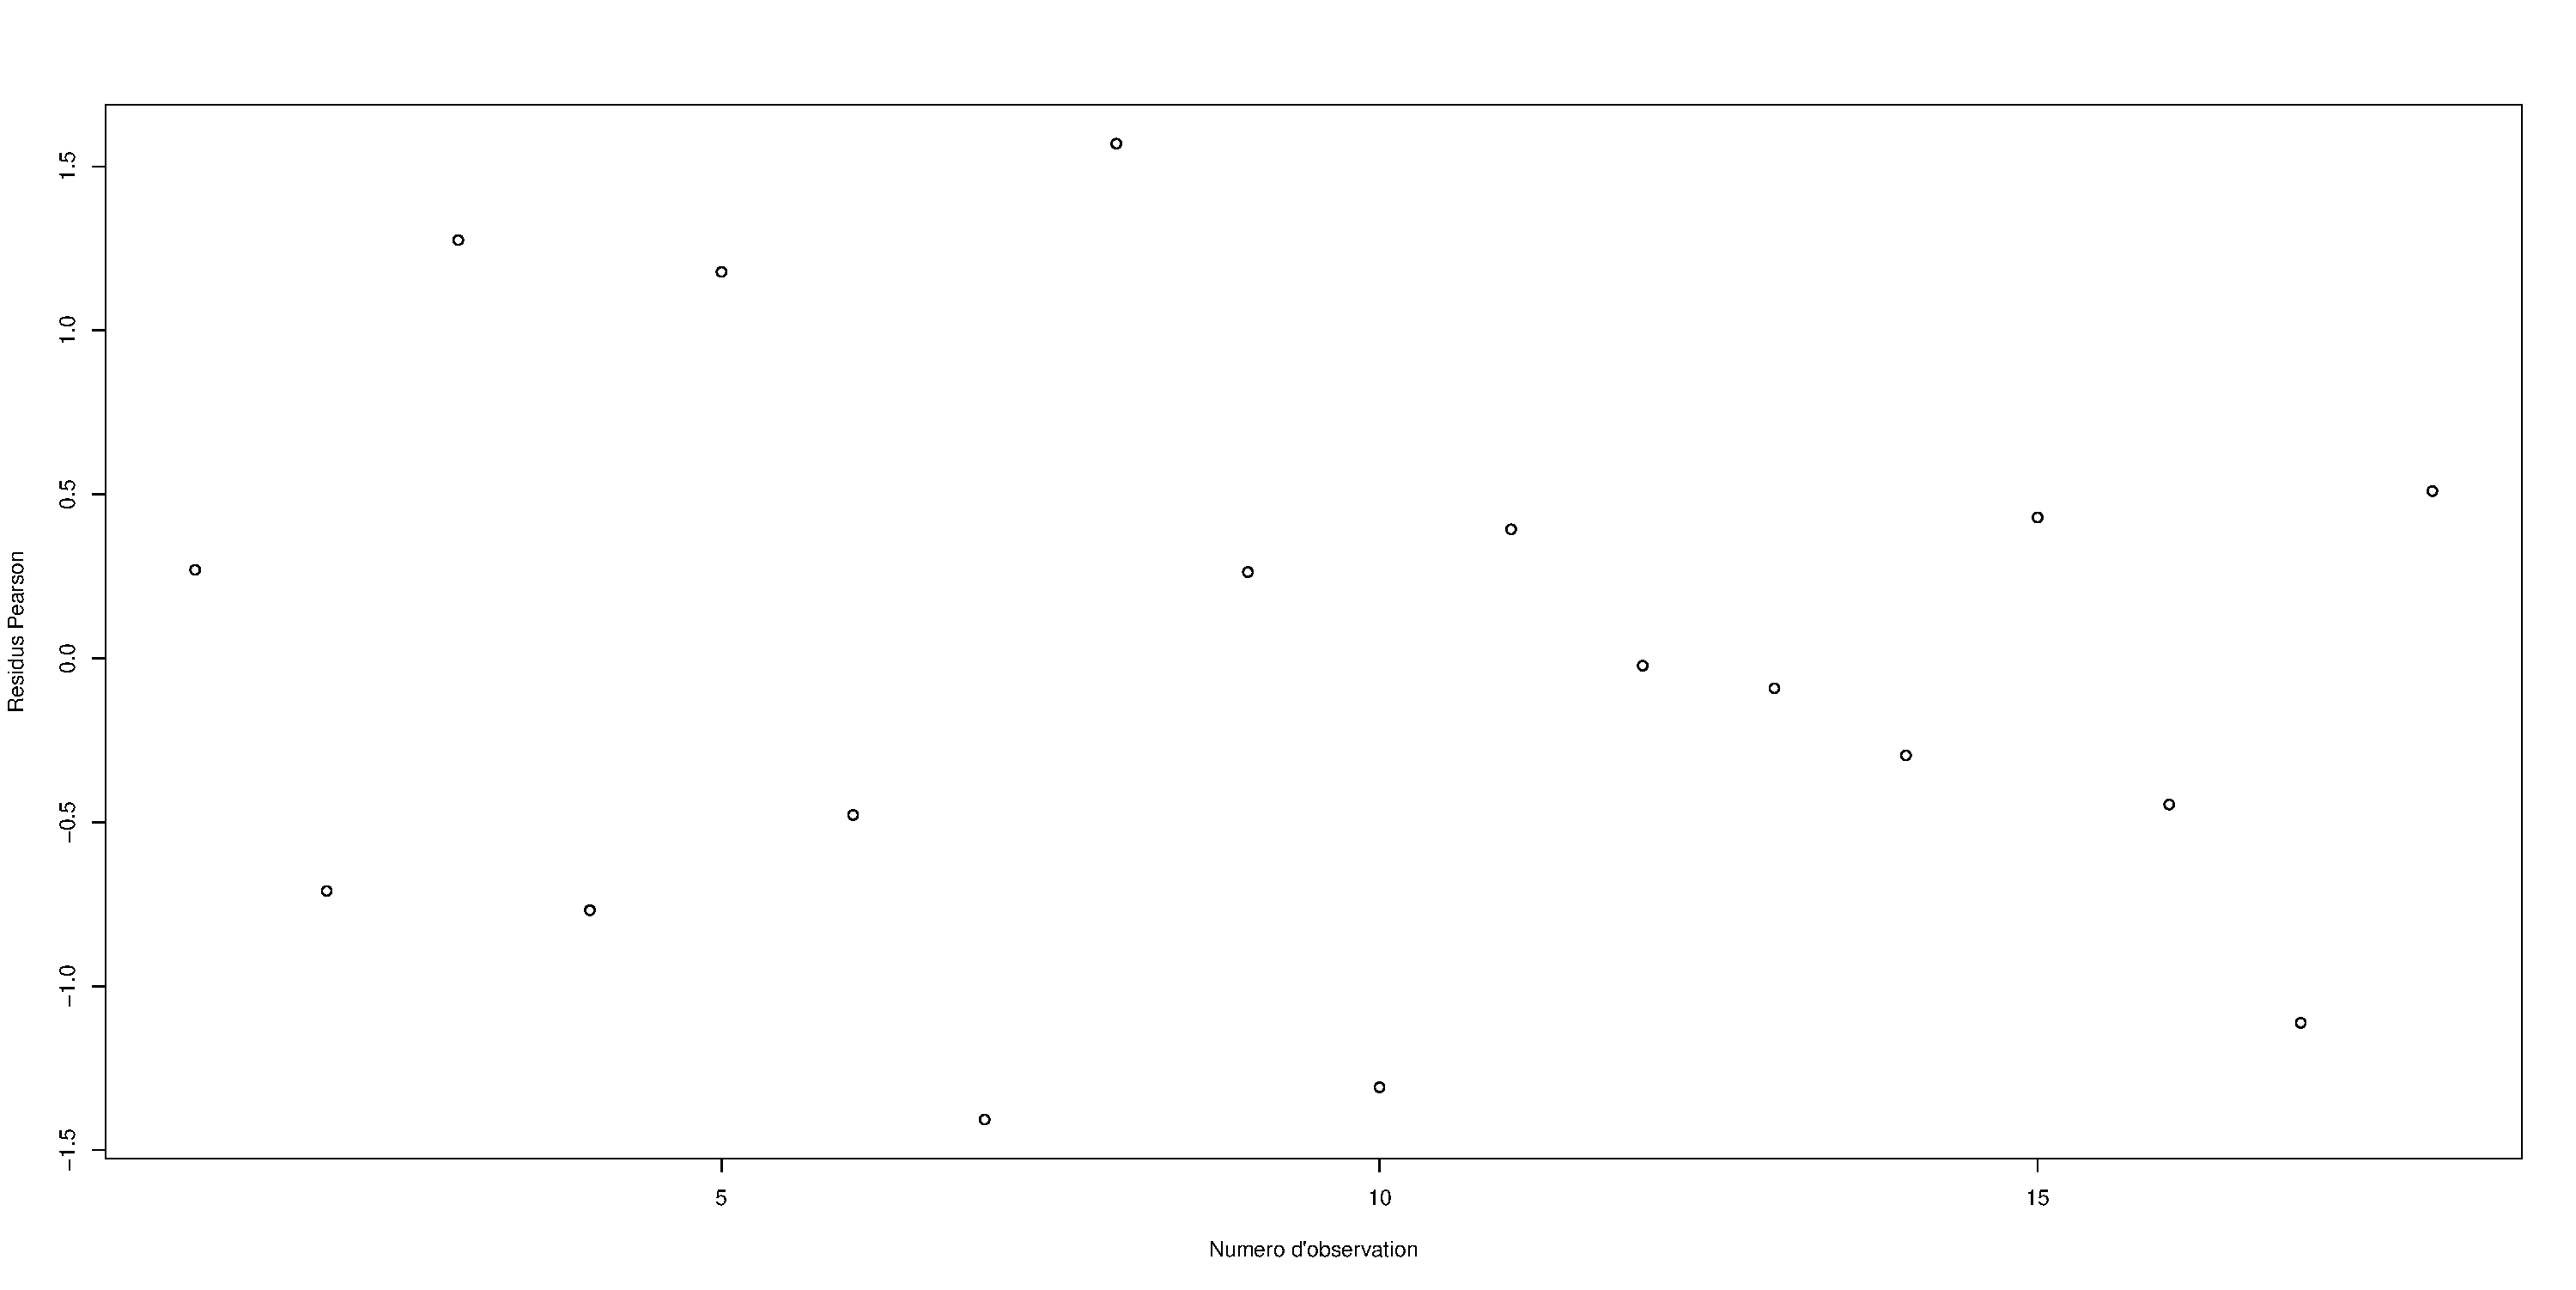
\includegraphics[scale=0.3]{Graphique6.pdf}
\end{center}

\noindent Si ces graphiques ont tendance horizentales mais plusieurs des valeurs sont sup\'erieures \`a 3 en valeur absolue, cela peut sugg\`erer la pr\'esence d'une extra-variabilit\'e. En effet, si la loi binomiale est bien sp\'ecifi\'ee, alors on a $E[Y_i]=m_i \pi_i$ et $Var[Y_i]=m_i \pi_i (1-\pi_i)$. Il arrive dans certaines situations o\`u on a $E[Y_i]=m_i \pi_i$ mais $Var[Y_i] > m_i \pi_i (1-\pi_i)$. On dit qu'on est en pr\'esence d'une extra-variabilit\'e ({\it overdispersion} en anglais). Dans cette situation, on pose $Var[Y_i] = \phi m_i \pi_i (1-\pi_i)$ et on estime $\phi$ par $\chi^2_P/(n-(p+1))$

\begin{verbatim}
> Pearson/(n-(p+1))
[1] 0.981905
\end{verbatim}

\noindent Dans notre cas, la valeur de $\chi^2_P/(n-(p+1))$ est tr\`es proche de 1. On ne d\'etecte aucune extra-variabilit\'e. Une solution \`a apporter en cas d'une \'eventuelle extra-variabilit\'e est de sp\'ecifier l'option \textsf{family=quasibinomial()} au lieu de \textsf{family=binomial()}. Cette solution consid\`ere une distribution pour $Y_i$ telle que $E[Y_i]=m_i \pi_i$ et $Var[Y_i]= \phi m_i \pi_i (1-\pi_i)$, avec $\phi>1$.

\noindent Pour v\'erifier la lin\'earit\'e $\eta_i=\beta_0+\beta_1 X_{i1}+\cdots+\beta_p X_{ip}$, on trace le nuage de points $\{(\hat\pi_i,\tilde\pi_i),i=1\cdots,n\}$. Ici, $\hat\pi_i=g^{-1}(\hat\eta_i)$ est l'estimateur de $\pi_i$ selon le mod\`ele consid\'er\'e et $\tilde\pi_i=y_i/m_i$ est l'estimateur empirique de $\pi_i$. Si la relation $\eta_i=\beta_0+\beta_1 X_{i1}+\cdots+\beta_p X_{ip}$ est bien sp\'ecifi\'ee, les estimateurs $\hat\pi_i$ et $\tilde\pi_i$ doivent \^etre proches et le nuage de points doit \^etre autour de la droite $x=y$.

\begin{verbatim}
> pi.chapeau <- fitted(modele)
> pi.tilde <- deposit$Killed/deposit$Number
> 
> plot(pi.chapeau,pi.tilde,type="p",xlim=c(0,1),ylim=c(0,1),
+      xlab="Estimateurs de pi selon le modele",ylab="Estimateurs empiriques de pi")
> abline(0,1,col="red")

\end{verbatim}

\noindent On obtient
\begin{center}
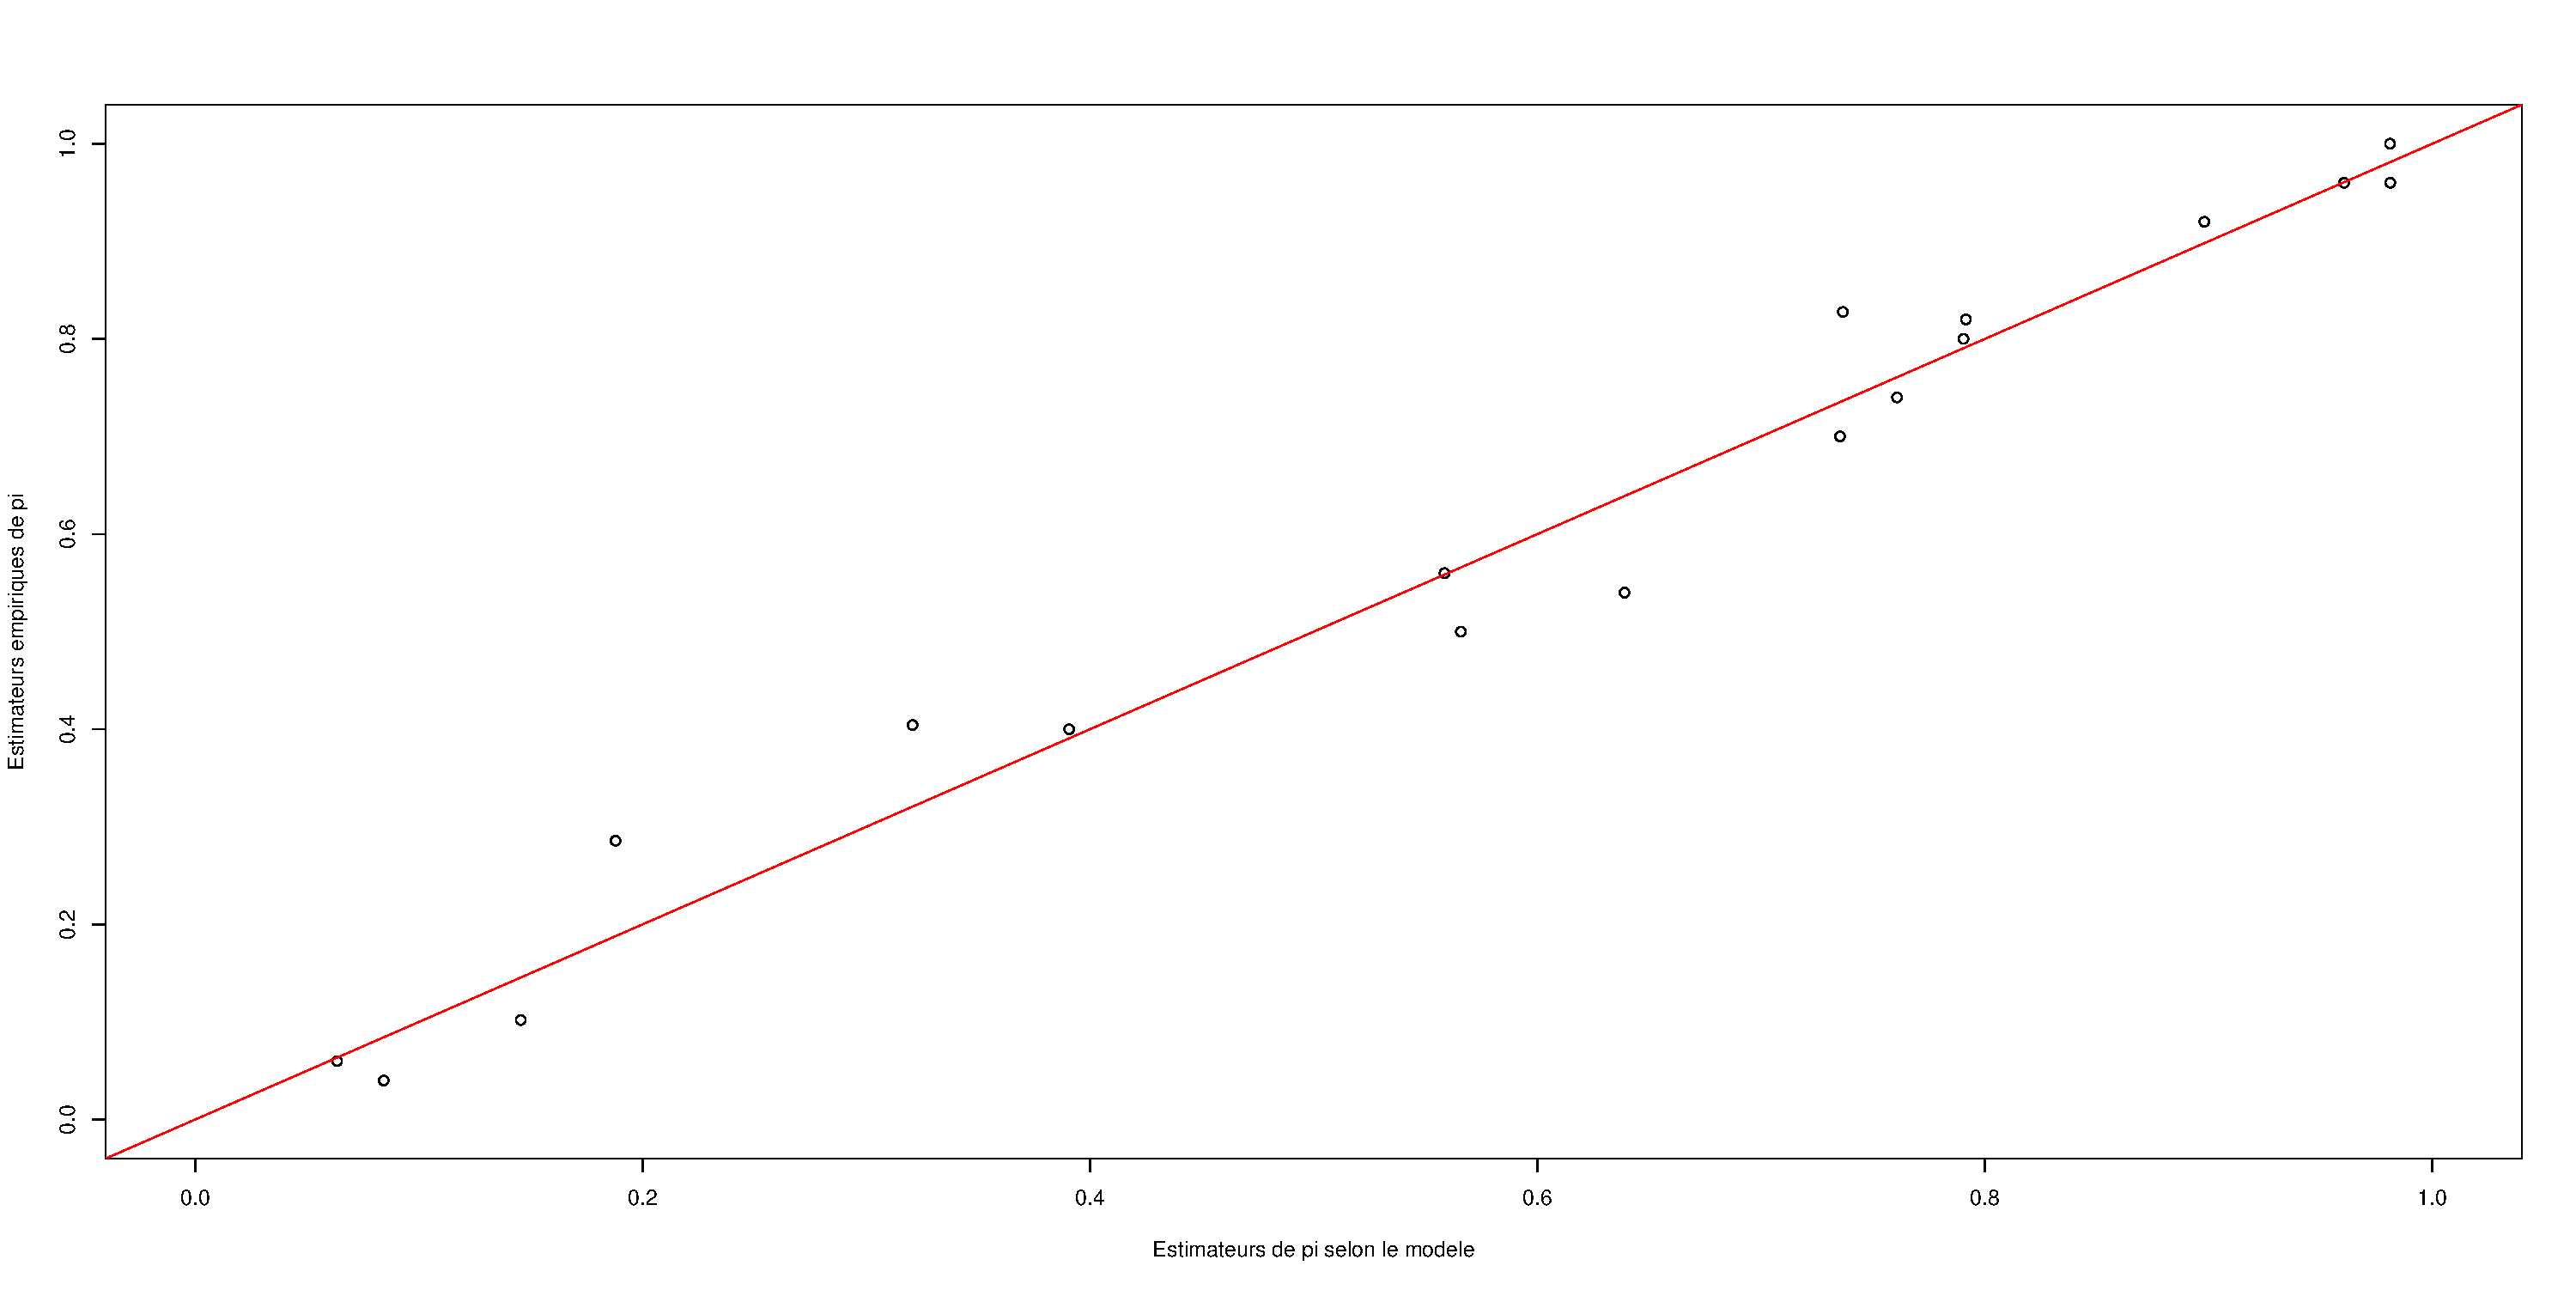
\includegraphics[scale=0.3]{Graphique7.pdf}
\end{center}

\subsection{Observations aberrantes \& valeurs influentes}

Le principe des observations aberrantes et valeurs influentes est identique pour les r\'egressions logistique et lin\'eaire. Les d\'efinitions des leviers des observations, des r\'esidus standardi\'es et studenti\'es sont diff\'erentes dans la cas d'une r\'egression logistique mais ces quantit\'es ont la m\^eme interpr\'etation et utilit\'e que dans le cadre d'une r\'egression lin\'eaire. C'est la m\^eme chose pour la distance de Cook, les DFBETAS, DFFITS et rapport de ratios. 

\subsection{Sp\'ecificit\'e, sensibilit\'e et courbe ROC}

Toutes les proc\'edures de diagnostique et validation de mod\`ele cit\'ees ci-haut ne sont valides que pour les donn\'ees group\'ees. Dans le cas de donn\'ees individuelles, c'est plus difficile d'\'evaluer l'ad\'equation des mod\`eles. Cependant, il est possible de mesurer la capacit\'e pr\'edictive du mod\`ele. 

\noindent Consid\'erons un mod\`ele avec des donn\'ees individuelles o\`u la variable r\'eponse est $Y_i \in \{0,1\}$, avec $P(Y_i=1)=\pi_i=g^{-1}(\nu_i)$, $\nu_i=\beta_0+\beta_1 X_{i1}+\cdots+\beta_p X_{ip}$ et $P(Y_i=0)=1-P(Y_i=1)$. On ajuste le mod\`ele, on obtient $\hat\beta_0$, $\hat\beta_1$, $\cdots$, $\hat\beta_p$ et on calcule les probabilit\'es pr\'edites $\hat\pi_i=g^{-1}(\hat\eta_i)$ avec $\hat\eta_i=\hat\beta_0+\hat\beta_1 X_{i1}+\cdots+\hat\beta_p X_{ip}$.

\noindent Fixons maintenant un r\'eel $u \in [0,1]$. Dans un contexte de classification, on pose $\hat y_i=1$ si $\hat\pi_i>u$ et $\hat y_i=0$ sinon. La valeur la plus utilis\'ee est $u=1/2$. On mesure la capacit\'e pr\'edictive du mod\`ele par la sp\'ecificit\'e et la sensibilit\'e, d\'efinies respectivement par $Spec = P(\hat y=0| y=0)$ et $Sens = P(\hat y=1| y=1)$. La sp\'ecificit\'e et la sensibilit\'e ref\`erent aux taux de vrais n\'egatifs et vrais positifs, respectivement. Plus ces valeurs sont proches de 1, plus grande est la capacit\'e pr\'edictive du mod\`ele. 

\noindent Pour un $u$ fix\'e, on calcule $\hat y_1, \cdots, \hat y_n$ et on estime la sp\'ecificit\'e et la sensibilit\'e du mod\`ele par 
\begin{eqnarray*}
\widehat{Spec}(u)&=&\frac{\sum_{i=1}^n I_{\{\hat y_i=0\}}}{\sum_{i=1}^n I_{\{(\hat y_i=0)\&(y_i=0)\}}} = \frac{\sum_{i=1}^n I_{\{\hat \pi_i < u \}}}{\sum_{i=1}^n I_{\{(\hat \pi_i < u)\&(y_i=0)\}}} \\
\widehat{Sens}(u)&=&\frac{\sum_{i=1}^n I_{\{\hat y_i=1\}}}{\sum_{i=1}^n I_{\{(\hat y_i=1)\&(y_i=1)\}}} = \frac{\sum_{i=1}^n I_{\{\hat \pi_i > u \}}}{\sum_{i=1}^n I_{\{(\hat \pi_i > u)\&(y_i=1)\}}}
\end{eqnarray*}

\noindent Faisons maintenant varier $u$ \`a l'int\'erieur d'une grille de $B$ points dans $[0,1]$: $\{u_1=0,u_1,u+2,\cdots,u_B=1\}$, avec $B$ suffisament grand.

\noindent Pour $b=0,1,\cdots,B$, on calcule $\widehat{Spec}(u_b)$ et $\widehat{Sens}(u_b)$. On trace le nuage de points $\{(1-\widehat{Spec}(u_b),\widehat{Sens}(u_b)),b=0,\cdots,B\}$. En reliant ces points, on obtient une courbe qu'on appelle la courbe ROC. On calcule l'aire sous cette courbe. Plus cette aire est grande, plus la capacit\'e pr\'edictive du mod\`ele est grande. 
$$
\mbox{Aire sous la courbe ROC} \in \begin{cases}
[0.9,1], & \mbox{ le mod\`ele est excellent} \\
[0.8,0.9], & \mbox{ le mod\`ele est bon} \\
[0.7,0.8], & \mbox{ le mod\`ele est moyen} \\
[0.6,0.7], & \mbox{ le mod\`ele est mauvais} \\
[0.7,0.8], & \mbox{ le mod\`ele est tr\`es faible.} \\
\end{cases}
$$

\noindent Consid\'erons maintenant le jeu de donn\'ees \textsf{quilpie} de la library \texttt{GLMsData} du logiciel \textrm{R}. Ce jeu de donn\'ees contient des observations de 1921 \`a 1988 de la quantit\'e de pluie mesur\'ee durant le mois de juillet \`a Quilpie en Australie. On consid\`ere une seule variable explicative $SOI$ qui mesure la pression atmosph\'erique. La variable r\'eponse ne peut prendre que 2 valeurs: 1 si la quanti\'e de pluie mesur\'ee est sup\'erieure \`a 10 millim\`etres et 0 sinon.

\begin{verbatim}
> if (!require("GLMsData")) install.packages("GLMsData")
Le chargement a nécessité le package : GLMsData
> library("GLMsData")#### Installer la librairie GLMsData
> 
> data(quilpie)
> 
> modele <- glm(y~SOI,family=binomial,data=quilpie)
> 
> if (!require("clinfun")) install.packages("clinfun")
Le chargement a nécessité le package : clinfun
> library("clinfun")#### Installer la librairie clinfun
> 
> courbe.roc <- roc.curve(marker=as.vector(fitted(modele)),
+                         status=quilpie$y,method=c("empirical"))
> print(courbe.roc)
  ROC curve with AUC = 0.7835498 and s.e. = 0.05651002 
\end{verbatim}

\noindent On obtient une aire sous la courbe de 0.78 avec une erreur-type de 0.056. On conclut que le mod\`ele est bon. On peut aussi tracer la courbe ROC:

\begin{verbatim}
> plot(courbe.roc)
\end{verbatim}

\noindent Et on obtient

\begin{center}
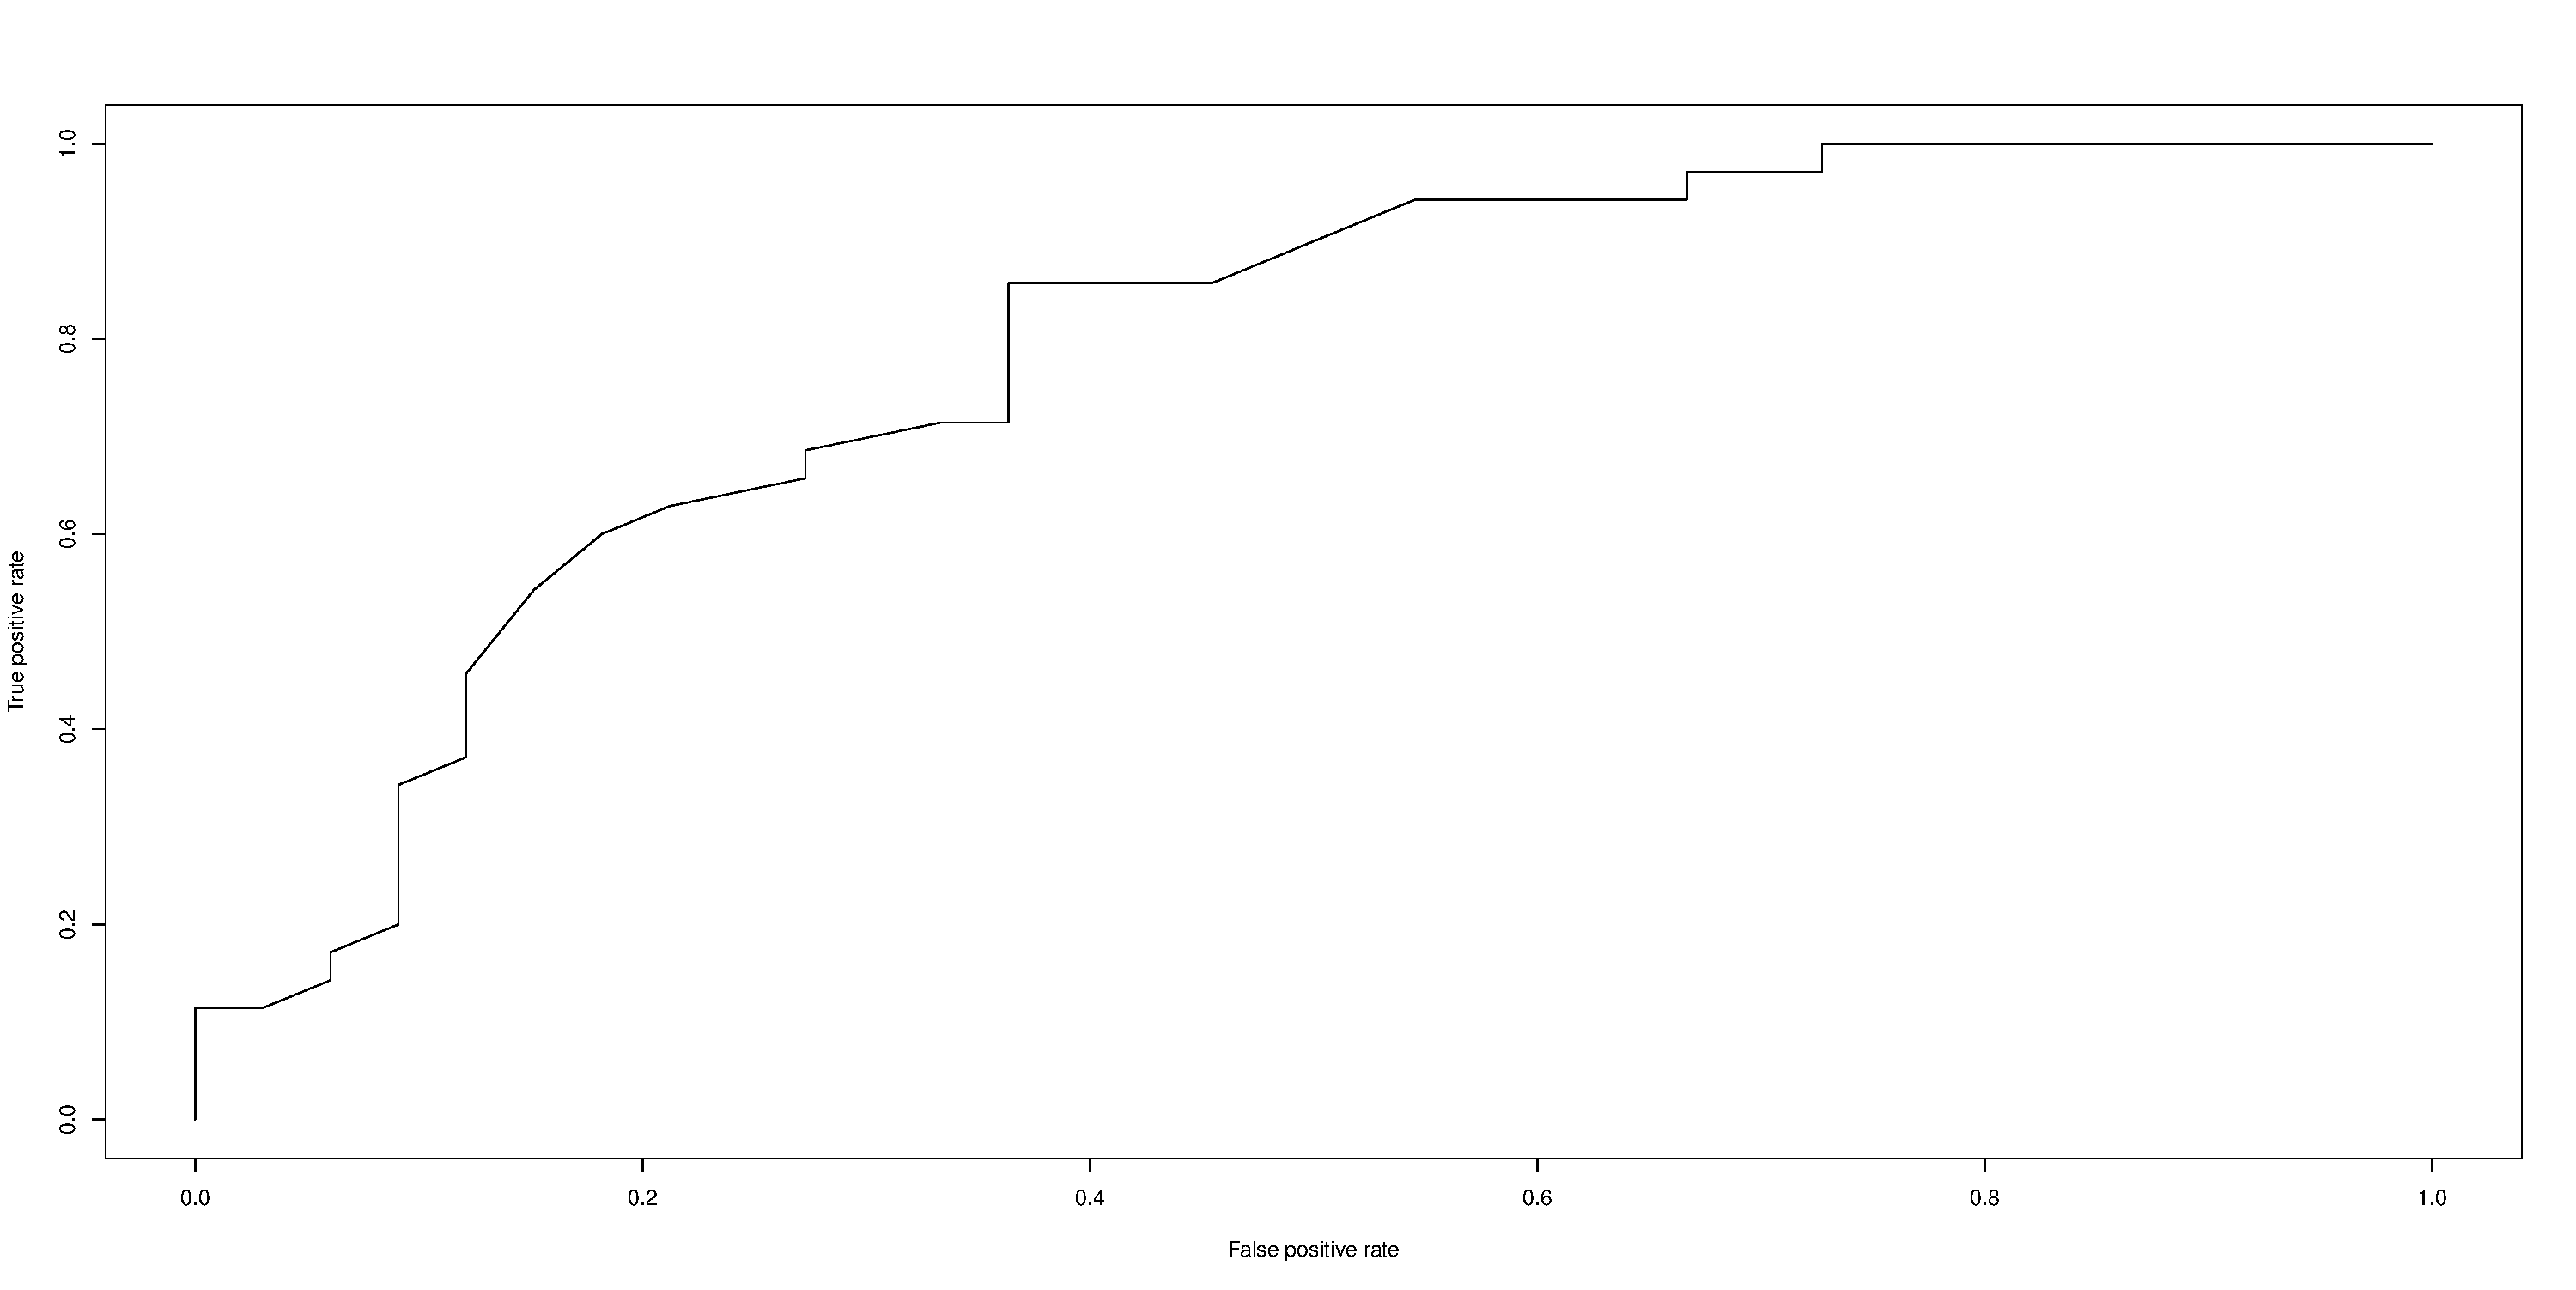
\includegraphics[scale=0.3]{Graphique8.pdf}
\end{center}


\end{document}
